\section{Experiments}

We evaluate the diagnosis recipe in three settings of increasing complexity: a synthetic logic task, an entity-binding task adapted from prior work \citep{gur2025mixing}, and an entangled factual recall setting based on the RAVEL benchmark \citep{huang2024ravel}. In each case, we begin with an existing causal abstraction obtained using a standard alignment method, observe that its global IIA is informative but non-perfect, and then apply our partitioning procedure to identify buckets with high within-bucket and low cross-bucket IIA. We finally test whether these partitions generalize beyond the analyzed sample and whether they suggest useful refinements to the original abstraction.
% We evaluate our method on three settings of increasing complexity: a synthetic logic task, an entity-binding task adapted from prior work, and an entangled factual recall setting based on the RAVEL benchmark. Across all experiments, we follow the same pipeline: we first construct a causal abstraction using existing alignment methods, observe that the resulting interchange intervention accuracy (IIA) is imperfect, and then apply our partitioning procedure to diagnose the source of this mismatch.

\subsection{Recursive Hypothesis Discovery in the Toy Logic Task}
\label{sec:logic-task-recursive}

Section~\ref{subsec:diagnosis-pipeline} established the first diagnosis pass for the toy logic task. Aligning \(o_5\) to position \(77\), layer \(7\) partitions the input space into two buckets, both of which have high within-bucket IIA but low cross-bucket IIA. The partition has a clear semantic interpretation: in the target bucket, \(o_4=o_1\wedge o_2\) is always \texttt{False}, whereas in the other bucket, \(o_4\) is always \texttt{True}. This shows that the candidate \(o_5\) alignment does not represent the full output uniformly. Instead, it separates two regimes of computation, suggesting that \(o_5\) should be refined into two variables, \(o_4\) and \(o_3\).

\begin{figure}[t]
    \centering
    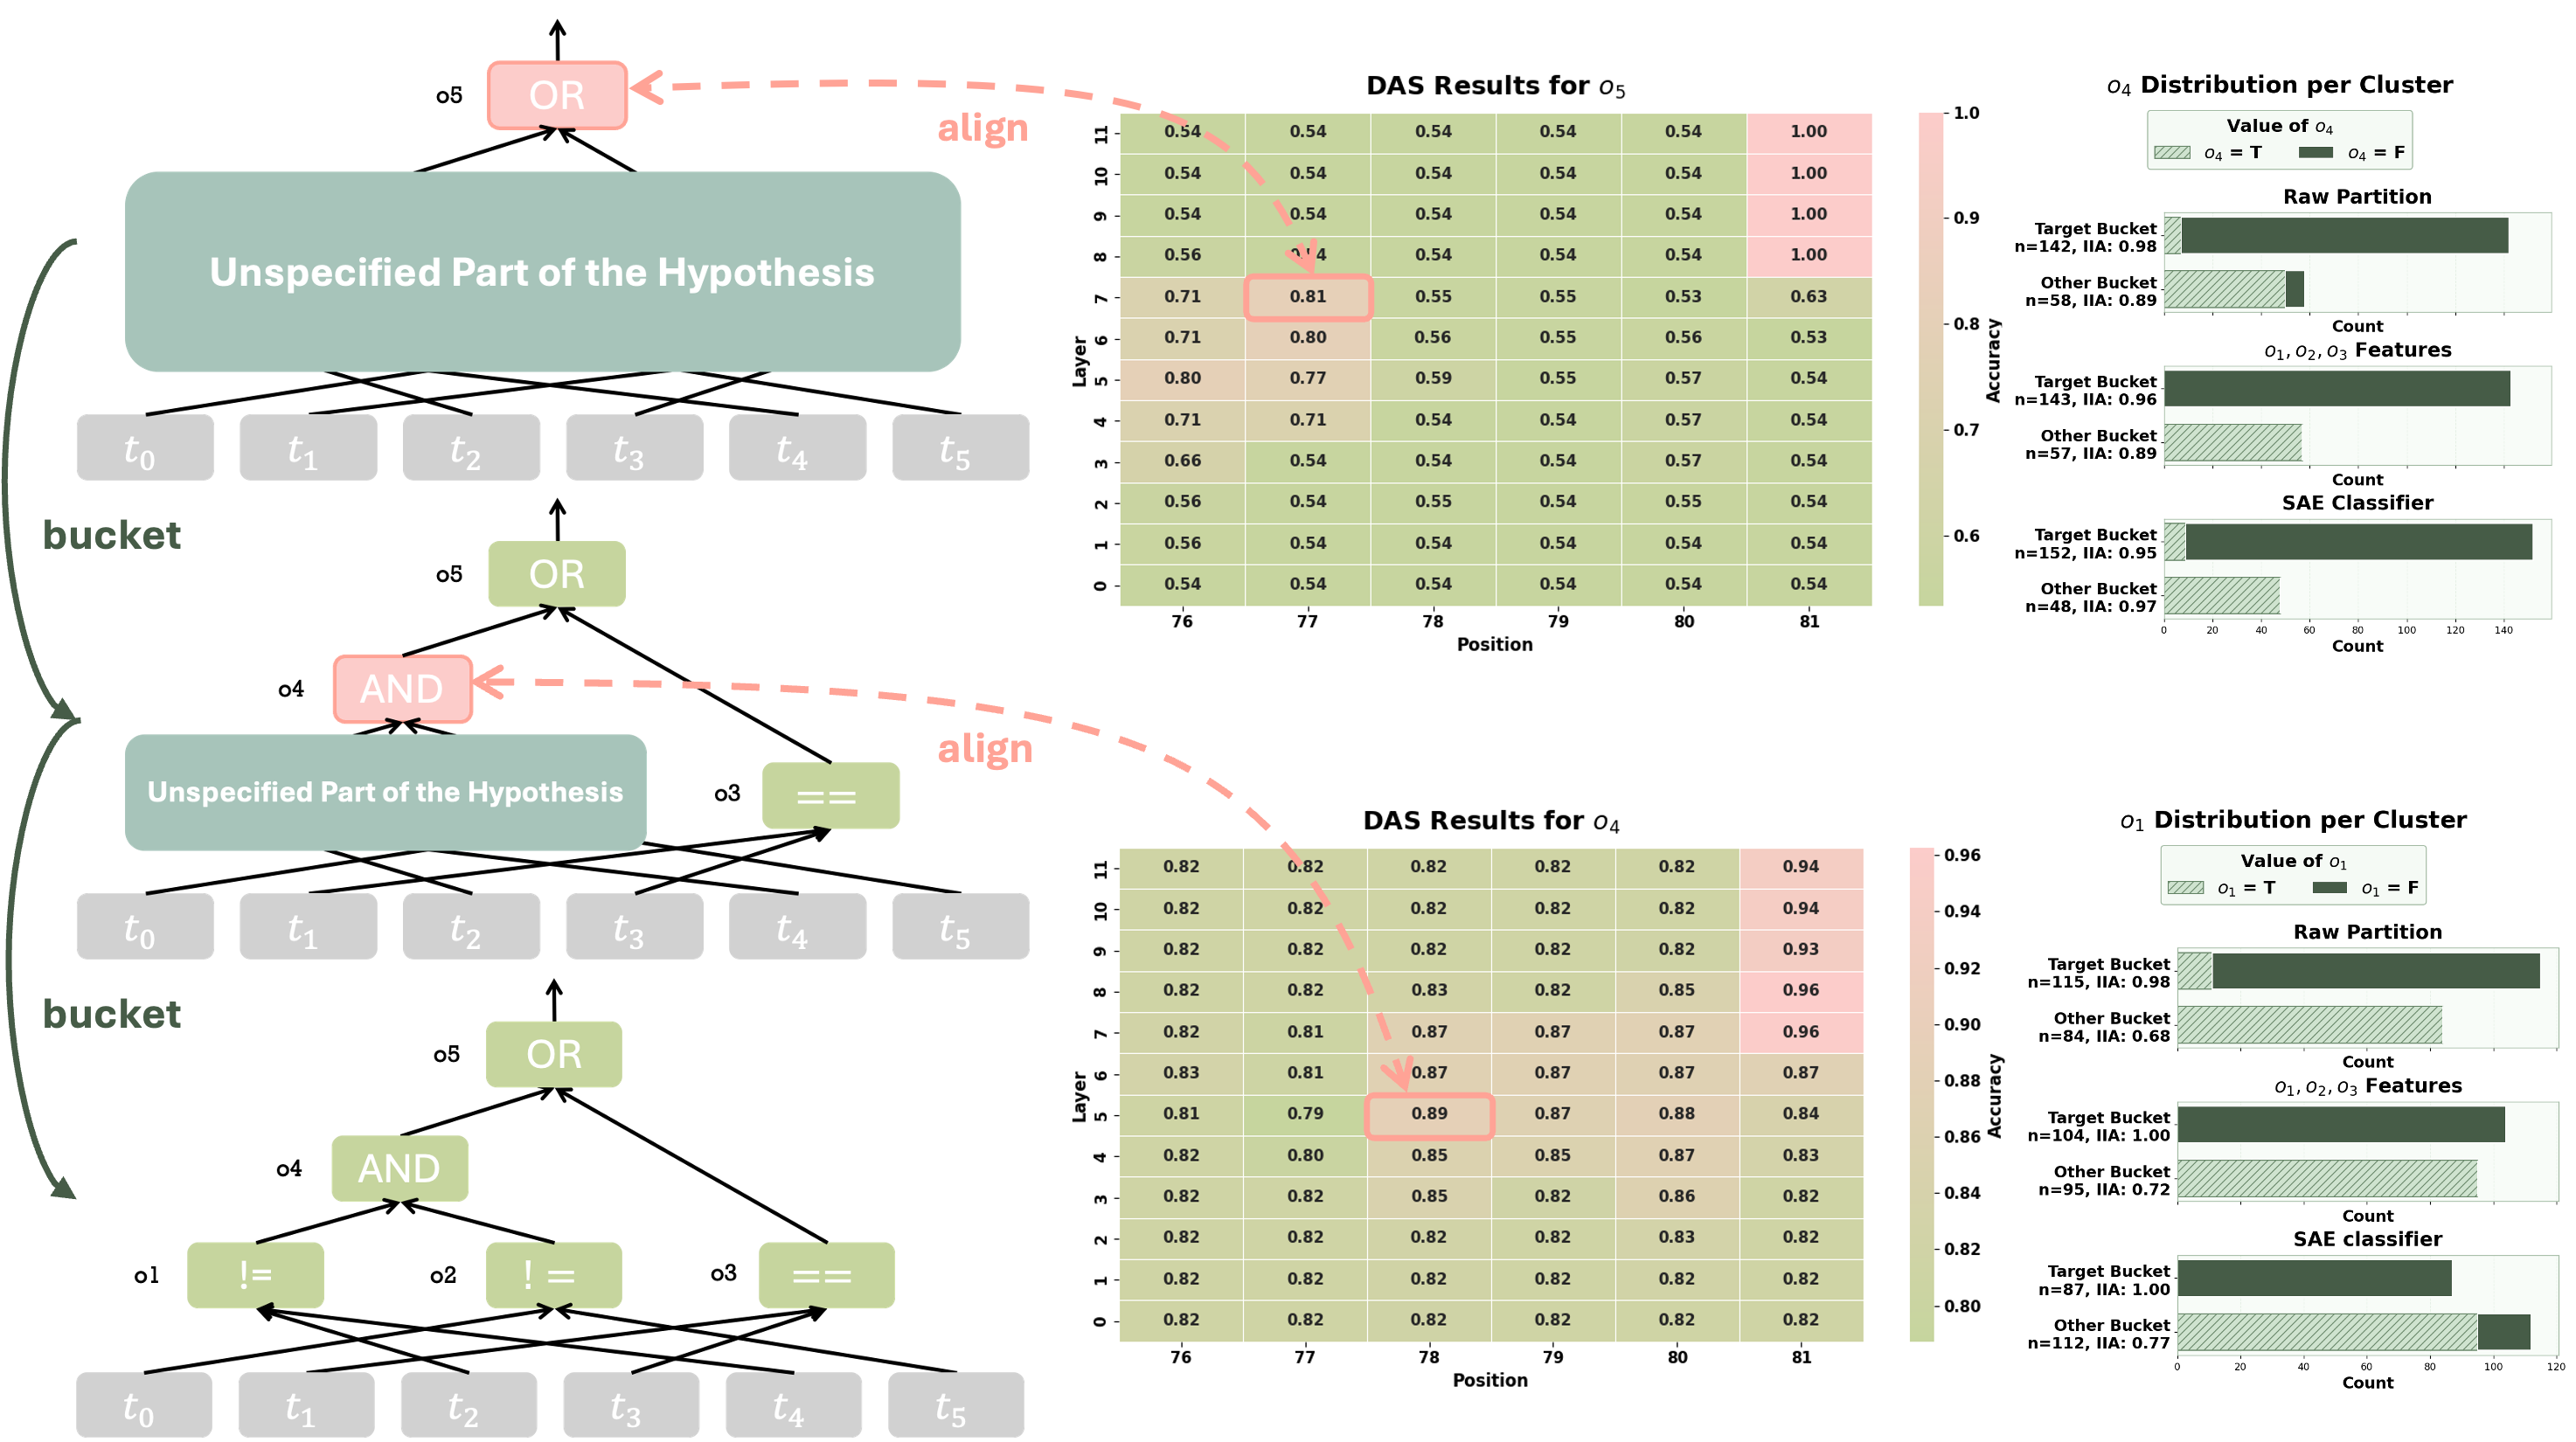
\includegraphics[width=1\linewidth]{figs/logic2_new.png}
    % \caption{ \textbf{Recursive Hypothesis Discovery}. The diagnosis recipe iteratively uncovers a model's latent hierarchical logic. \textbf{Left}: An initial underspecified hypothesis targeting only the output $o_5$ reveals a partition that depends on the missing intermediate variable $o_4$. \textbf{Middle}: Promoting $o_4$ to an explicit variable in the hypothesis enables a second diagnosis pass at a refined internal site. \textbf{Right}: Partitioning the new $o_4$ alignment recovers the primitive component $o_1$, successfully reconstructing the full causal hierarchy from scratch.}
    \caption{\textbf{Recursive hypothesis discovery in the toy logic task.} \textbf{Top:} Diagnosing the candidate \(o_5\) alignment at position \(77\), layer \(7\) partitions the input space into two high-IIA buckets separated by the latent variable \(o_4=o_1\wedge o_2\). \textbf{Middle:} After promoting \(o_4\) to an explicit variable, DAS identifies both a near-perfect signal at position \(81\), layer \(7\) and a non-trivial earlier signal at position \(78\), layer \(5\). \textbf{Bottom:} Diagnosing the earlier \(o_4\) signal reveals \(o_1\) as the next missing component, recovering the complete hierarchy.}
    \label{fig:logic_recur}
\end{figure}

We then apply the same diagnosis procedure to \(o_4\). DAS identifies a near-perfect signal for \(o_4\) at position \(81\), layer \(7\), indicating that the completed \(o_4\) computation can be localized there, and also a non-trivial above-baseline signal at position \(78\), layer \(5\). We align \(o_4\) to this earlier site and repeat the bucketing step. The resulting partition again yields two buckets with high within-bucket IIA, and in the target bucket \(o_1\) is always \texttt{False}. This shows that the earlier \(o_4\) signal can itself be decomposed into the primitive components \(o_1\) and \(o_2\). Classifiers trained on both hand-labeled features and SAE features generalize these bucket assignments well, and their predictions are largely consistent, indicating that the discovered boundaries reflect stable structure rather than artifacts of a finite intervention graph.

Taken together, these two passes recover the hierarchy \(o_1,o_2,o_3 \rightarrow o_4 \rightarrow o_5\). Starting from the output variable alone, recursive diagnosis spells out the full high-level causal hypothesis from top to bottom. In particular, it shows that the model solves the task via the intended factorization \(y=(o_1\wedge o_2)\vee o_3\), rather than the extensionally equivalent alternative \(y=(o_1\vee o_3)\wedge(o_2\vee o_3)\). Consistent with this picture, alignment search over all variables localizes \(o_3\) at position \(77\), layer \(7\), and \(o_1\) at position \(78\), layer \(5\) (Appendix~\ref{appendix:logic}).

% Section~\ref{subsec:diagnosis-pipeline} showed how a single diagnosis pass, starting from an underspecified output-only hypothesis, reveals a structured failure mode and identifies the conjunction branch \(o_4=o_1\wedge o_2\) as a missing intermediate variable. We now treat that result not as an endpoint, but as the starting point of iterative refinement. Once the first pass suggests that the boundary between the well-interpreted and under-interpreted regions is governed by \(o_4\), the natural next step is to promote \(o_4\) from an implicit condition to an explicit variable in the high-level model. This yields the refined hypothesis
% \[
% o_5 = o_4 \vee o_3,
% \qquad\text{where}\qquad
% o_4 = o_1 \wedge o_2.
% \]
% The key question is whether this refinement is merely descriptive, or whether the same diagnosis procedure can be reapplied to \(o_4\) itself such that it will then be possible to continue to expose additional internal structure.

% To test this, we run a second diagnostic pass targeting \(o_4\). We first identify a candidate alignment for \(o_4\), located at position \(75\), layer \(5\), and then repeat exactly the same partition-and-classify procedure used in the first pass. The results are shown in \cref{fig:logic_recur}. For the original \(o_5\) partition, both interpretable features \((o_1,o_2,o_3)\) and SAE features generalize the bucket structure well, confirming that the first diagnosis is not an artifact of a finite intervention graph. More importantly, once the pipeline is reapplied to \(o_4\), both feature spaces again recover a highly structured partition, and the good bucket reaches \(100\%\) IIA. The interpretable classifier in this second pass assigns its dominant weight to \(o_1\), while the remaining coefficients are comparatively small, indicating that the newly surfaced variable \(o_4\) can itself be decomposed into more primitive components.

% Taken together, the two passes recover the intended hierarchy:
% \[
% o_1,\;o_2,\;o_3
% \;\longrightarrow\;
% o_4=o_1\wedge o_2
% \;\longrightarrow\;
% o_5=o_4\vee o_3.
% \]
% In other words, starting from a coarse hypothesis containing only the final output variable, recursive diagnosis progressively spells out the intermediate variables needed to explain the model's behavior. This is the constructive aspect of the method: the first diagnosis does not merely say that the abstraction is imperfect, but identifies how it should be refined, and the same recipe can then be reused on the refined hypothesis.

% The toy logic task therefore serves as a proof of concept for iterative hypothesis discovery. Rather than merely scoring a fixed abstraction, the recipe supports a step-by-step process in which a middling global IIA is converted into a local structural diagnosis, the diagnosis proposes a missing variable, and reapplying the same procedure to that newly reified variable recovers a fuller causal account of the computation.

% \begin{table}[ht]
% \centering
% \caption{Recursive discovery results for the toy logic task. The first pass diagnoses an underspecified hypothesis for \(o_5\); the second pass reapplies the same procedure to the newly introduced variable \(o_4\).}
% \label{tab:logic-classifier-recursive}
% \begin{tabular}{llcccc}
% \toprule
% \textbf{Target} & \textbf{Feature Space} & \textbf{Test Acc.} & \textbf{Overall IIA} & \textbf{Bad Bucket} & \textbf{Good Bucket} \\
% \midrule
% \multirow{2}{*}{$o_5$} & Interpretable (\(o_1,o_2,o_3\)) & \(97.5\%\) & \(68.0\%\) & \(89.0\%\) & \(96.0\%\) \\
% & SAE & \(85.0\%\) & \(68.0\%\) & \(97.0\%\) & \(95.3\%\) \\
% \midrule
% \multirow{2}{*}{$o_4$} & Interpretable (\(o_1,o_2,o_3\)) & \(92.5\%\) & \(85.6\%\) & \(71.9\%\) & \(100.0\%\) \\
% & SAE & \(92.5\%\) & \(85.6\%\) & \(76.6\%\) & \(100.0\%\) \\
% \bottomrule
% \end{tabular}
% \end{table}

% \subsection{A Toy Logic Task}

% \textbf{Task and input space.}
% We begin with a controlled synthetic task in which the target computation is known exactly. We fine-tune a 
% 12-layer GPT-2-small model (\(\sim\)117M parameters) to perform a Boolean reasoning task over six input tokens 
% \(t_0,\dots,t_5\). The target label is
% \[
% o_5 \;=\; \bigl((t_2 \neq t_4)\wedge (t_0 \neq t_5)\bigr)\;\vee\;(t_1 = t_3).
% \]
% For clarity, we name the intermediate variables
% \[
% o_1 := (t_2 \neq t_4), \qquad
% o_2 := (t_0 \neq t_5), \qquad
% o_3 := (t_1 = t_3), \qquad
% o_4 := o_1 \wedge o_2,
% \]
% so that the final output is \(o_5 = o_4 \vee o_3\).\footnote{Trained only on input-output pairs without symbolic supervision, the model may implement any extensionally equivalent Boolean factorization (e.g., $y = (o_1 \wedge o_2) \vee o_3$ vs. $y = (o_1 \vee o_3) \wedge (o_2 \vee o_3)$). This allows us to test which specific internal algorithm our method recovers, rather than merely evaluating predictive accuracy.} The dataset is 
% generated so that \(o_1,o_2,o_3\) are each true with probability \(0.5\), yielding an approximately balanced 
% input space over the eight possible assignments of the three primitive Boolean variables. We train on a 
% synthetic dataset of size \(20{,}48\), and the resulting model achieves $99.7\%$ test 
% accuracy.

% \begin{figure}[ht]
%     \centering
%     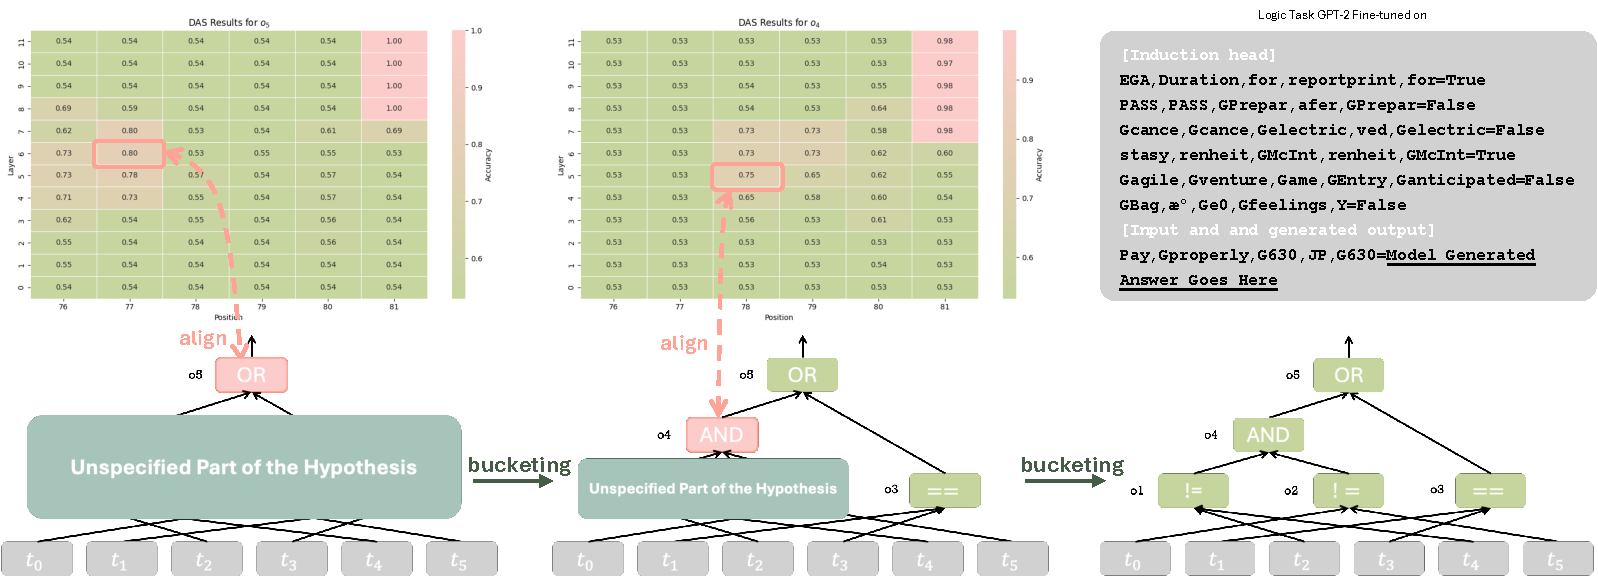
\includegraphics[width=\linewidth]{figs/logic_task.pdf}
%     \caption{logic task}
%     \label{fig:placeholder}
% \end{figure}

% % \begin{figure}[ht]
% %     \centering
% %     % First Subfigure: o4 Heatmap
% %     \begin{subfigure}[b]{0.48\linewidth}
% %         \centering
% %         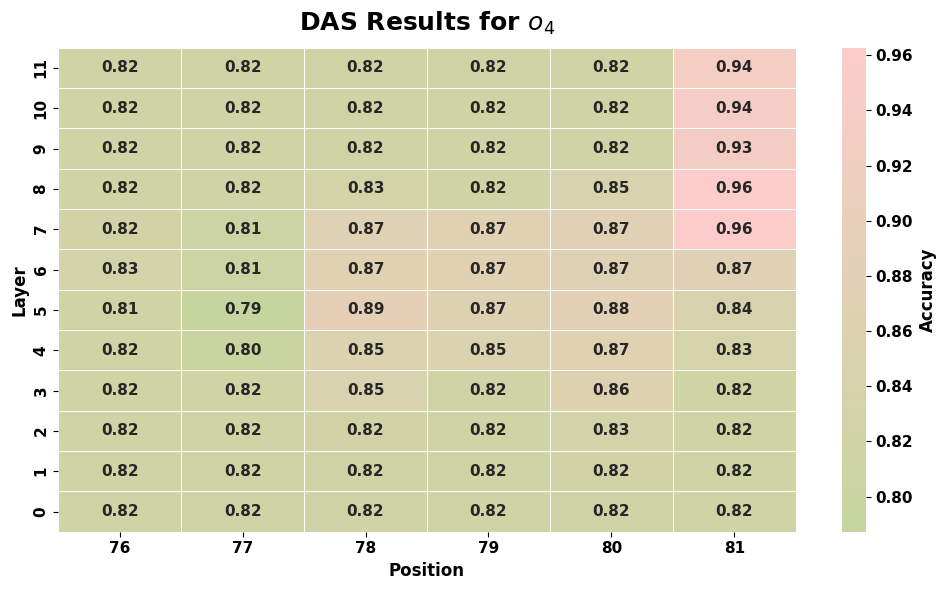
\includegraphics[width=\linewidth]{figs/das_heatmap_o4.png}
% %         \caption{DAS results for intermediate variable $o_4$.}
% %         \label{fig:das_o4}
% %     \end{subfigure}
% %     \hfill % Adds horizontal space between the two images
% %     % Second Subfigure: o5 Heatmap
% %     \begin{subfigure}[b]{0.48\linewidth}
% %         \centering
% %         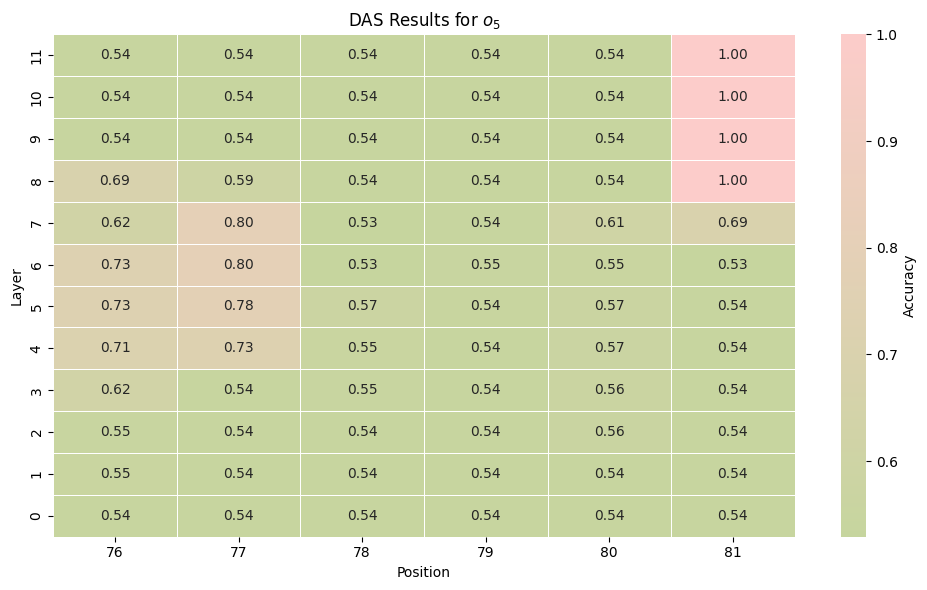
\includegraphics[width=\linewidth]{figs/das_heatmap_o5.png}
% %         \caption{DAS results for final output variable $o_5$.}
% %         \label{fig:das_o5}
% %     \end{subfigure}
% %     \caption{Interchange Intervention Accuracy (IIA) heatmaps across layers and token positions for the Boolean logic task.}
% %     \label{fig:das_combined_results}
% % \end{figure}

% \textbf{Alignment and preliminary evaluation.} 
% To evaluate the diagnostic utility of our method, we intentionally begin with an underspecified high-level hypothesis containing only the final output variable $o_5$. We perform DAS over residual-stream representations across all token positions and layers. As expected, DAS identifies a near-perfect alignment at the final output position (token 81), where the representations in the final four layers achieve $100\%$ IIA.

% However, DAS also surfaces an earlier candidate alignment at position 77 (corresponding to $t_3$) in layer 7, yielding a moderate IIA of approximately $0.78$. While this performance significantly exceeds the $0.5$ binary baseline, it is insufficient to support the claim of a globally faithful encoding. At this stage, the aggregate IIA score remains an ambiguous signal: it cannot distinguish whether the representation is inherently noisy, faithful only on a structured input subspace, or if the coarse high-level hypothesis is collapsing distinct internal computations. This ambiguity motivates the application of our partitioning procedure to localize and characterize the source of the alignment failure.

% \textbf{Partitioning the Input Space.}
% We apply our partitioning procedure to the candidate alignment at position 77, layer 7, which targets the high-level variable $o_5$. By constructing the Interchangeability Graph over $\mathcal{I}_{\mathrm{correct}}$ and partitioning it into two clusters, we immediately identify the structural source of the intermediate $0.78$ IIA score. In the ``well-interpreted'' bucket, nearly all inputs satisfy $o_4 = (o_1 \wedge o_2) = \text{False}$. In this region of the input space, the target expression $o_5 = o_4 \vee o_3$ simplifies to $o_5 = o_3$. Consequently, an internal representation that tracks only $o_3$ appears locally faithful to the full output variable. 

% Conversely, in the under-interpreted bucket, $o_4$ is almost exclusively \text{True}. In this subspace, the final output is driven by the conjunction branch, and a feature that fails to capture $o_1 \wedge o_2$ cannot reproduce the correct counterfactual behavior of $o_5$. This diagnosis reveals that the alignment at position 77 is not a noisy representation of the full output, but rather a \emph{partial interpretation}: it remains clean and faithful only within the subspace where the alternate computational branch is inactive. Furthermore, this result favors the hypothesized factorization $o_5 = (o_1 \wedge o_2) \vee o_3$ over extensionally equivalent alternatives, as the discovered partition is explicitly organized by the truth value of the intermediate variable $o_4$.

% \textbf{Generalization through classification.}
% To evaluate whether the discovered partitions recover the underlying structure, we train linear classifiers to predict bucket membership for unseen inputs. We first examine the $o_5$ candidate alignment at position 77, layer 7, which exhibits a moderate global IIA of $61.2\%$. As shown in Table~\ref{tab:logic-classifier-recursive}, classifiers using both \emph{interpretable features} $(o_1, o_2, o_3)$ and \emph{SAE features} \cite{bloom2024saetrainingcodebase} (SAE activations from layer 8, position 81) generalize the partition with high accuracy ($97.5\%$ and $85.0\%$, respectively). For the interpretable classifier, the dominant absolute coefficients are assigned to $o_2$ ($-2.95$) and $o_1$ ($-2.47$). This result confirms that the boundary between the well-interpreted and under-interpreted regions is governed by the state of the conjunction branch $o_4 = o_1 \wedge o_2$, identifying it as the missing component in our initial hypothesis.

% We then recursively apply the diagnosis recipe to the latent variable $o_4$ at position 75, layer 5. For this alignment, which exhibits a global IIA of $75.5\%$, both feature sets achieve a test accuracy of $92.5\%$. This secondary partition successfully isolates a perfectly interpreted subspace ($100\%$ IIA). Notably, the interpretable classifier identifies $o_1$ (coefficient $4.04$) as the primary governing factor, while the coefficients for other components remain negligible. This recursive decomposition corroborates our previous finding: by isolating subspaces where specific causal factors are inactive, our method can systematically expose and characterize a model's latent hierarchical logic.

% \begin{table}[ht]
% \centering
% \caption{Recursive discovery results: Classifier performance and IIA per bucket for both $o_5$ and $o_4$ partitions.}
% \label{tab:logic-classifier-recursive}
% \begin{tabular}{llcccc}
% \toprule
% \textbf{Target} & \textbf{Feature Space} & \textbf{Test Acc.} & \textbf{Overall IIA} & \textbf{Bad Bucket} & \textbf{Good Bucket} \\
% \midrule
% \multirow{2}{*}{$o_5$} & Interpretable ($o_1, o_2, o_3$) & $97.5\%$ & $68.0\%$ & $89.0\%$ & $96.0\%$ \\
%  & SAE  & $85.0\%$ & $68.0\%$ & $97.0\%$ & $95.3\%$ \\
% \midrule
% \multirow{2}{*}{$o_4$} & Interpretable ($o_1, o_2, o_3$) & $92.5\%$ & $85.6\%$ & $71.9\%$ & $100.0\%$ \\
%  & SAE  & $92.5\%$ & $85.6\%$ & $76.6\%$ & $100.0\%$ \\
% \bottomrule
% \end{tabular}
% \end{table}

% \textbf{Takeaway.}
% This toy experiment validates our diagnostic recipe by transforming an ambiguous global IIA score into a precise local diagnosis. While an underspecified hypothesis targeting only the output variable ($o_5$) yields a middling score that is difficult to interpret in isolation, partitioning the input space reveals that the alignment is perfectly faithful on a structured subspace. The accompanying classifier demonstrates that this partition is generalizable, providing a practical signal for identifying when an abstraction is trustworthy.

% Crucially, this diagnostic process is constructive rather than merely descriptive. By isolating the failure modes of the $o_5$ alignment, the method directly identifies the missing intermediate variable $o_4$. Through recursive application, $o_4$ is further decomposed into its primitive components $o_1$ and $o_2$. In this manner, the logic task demonstrates that our framework does more than evaluate existing abstractions—it actively assists in \emph{build}ing high-level hypotheses from scratch by iteratively exposing latent causal structure.

\subsection{Entity Binding Task}

\begin{figure}[!ht]
    \centering
    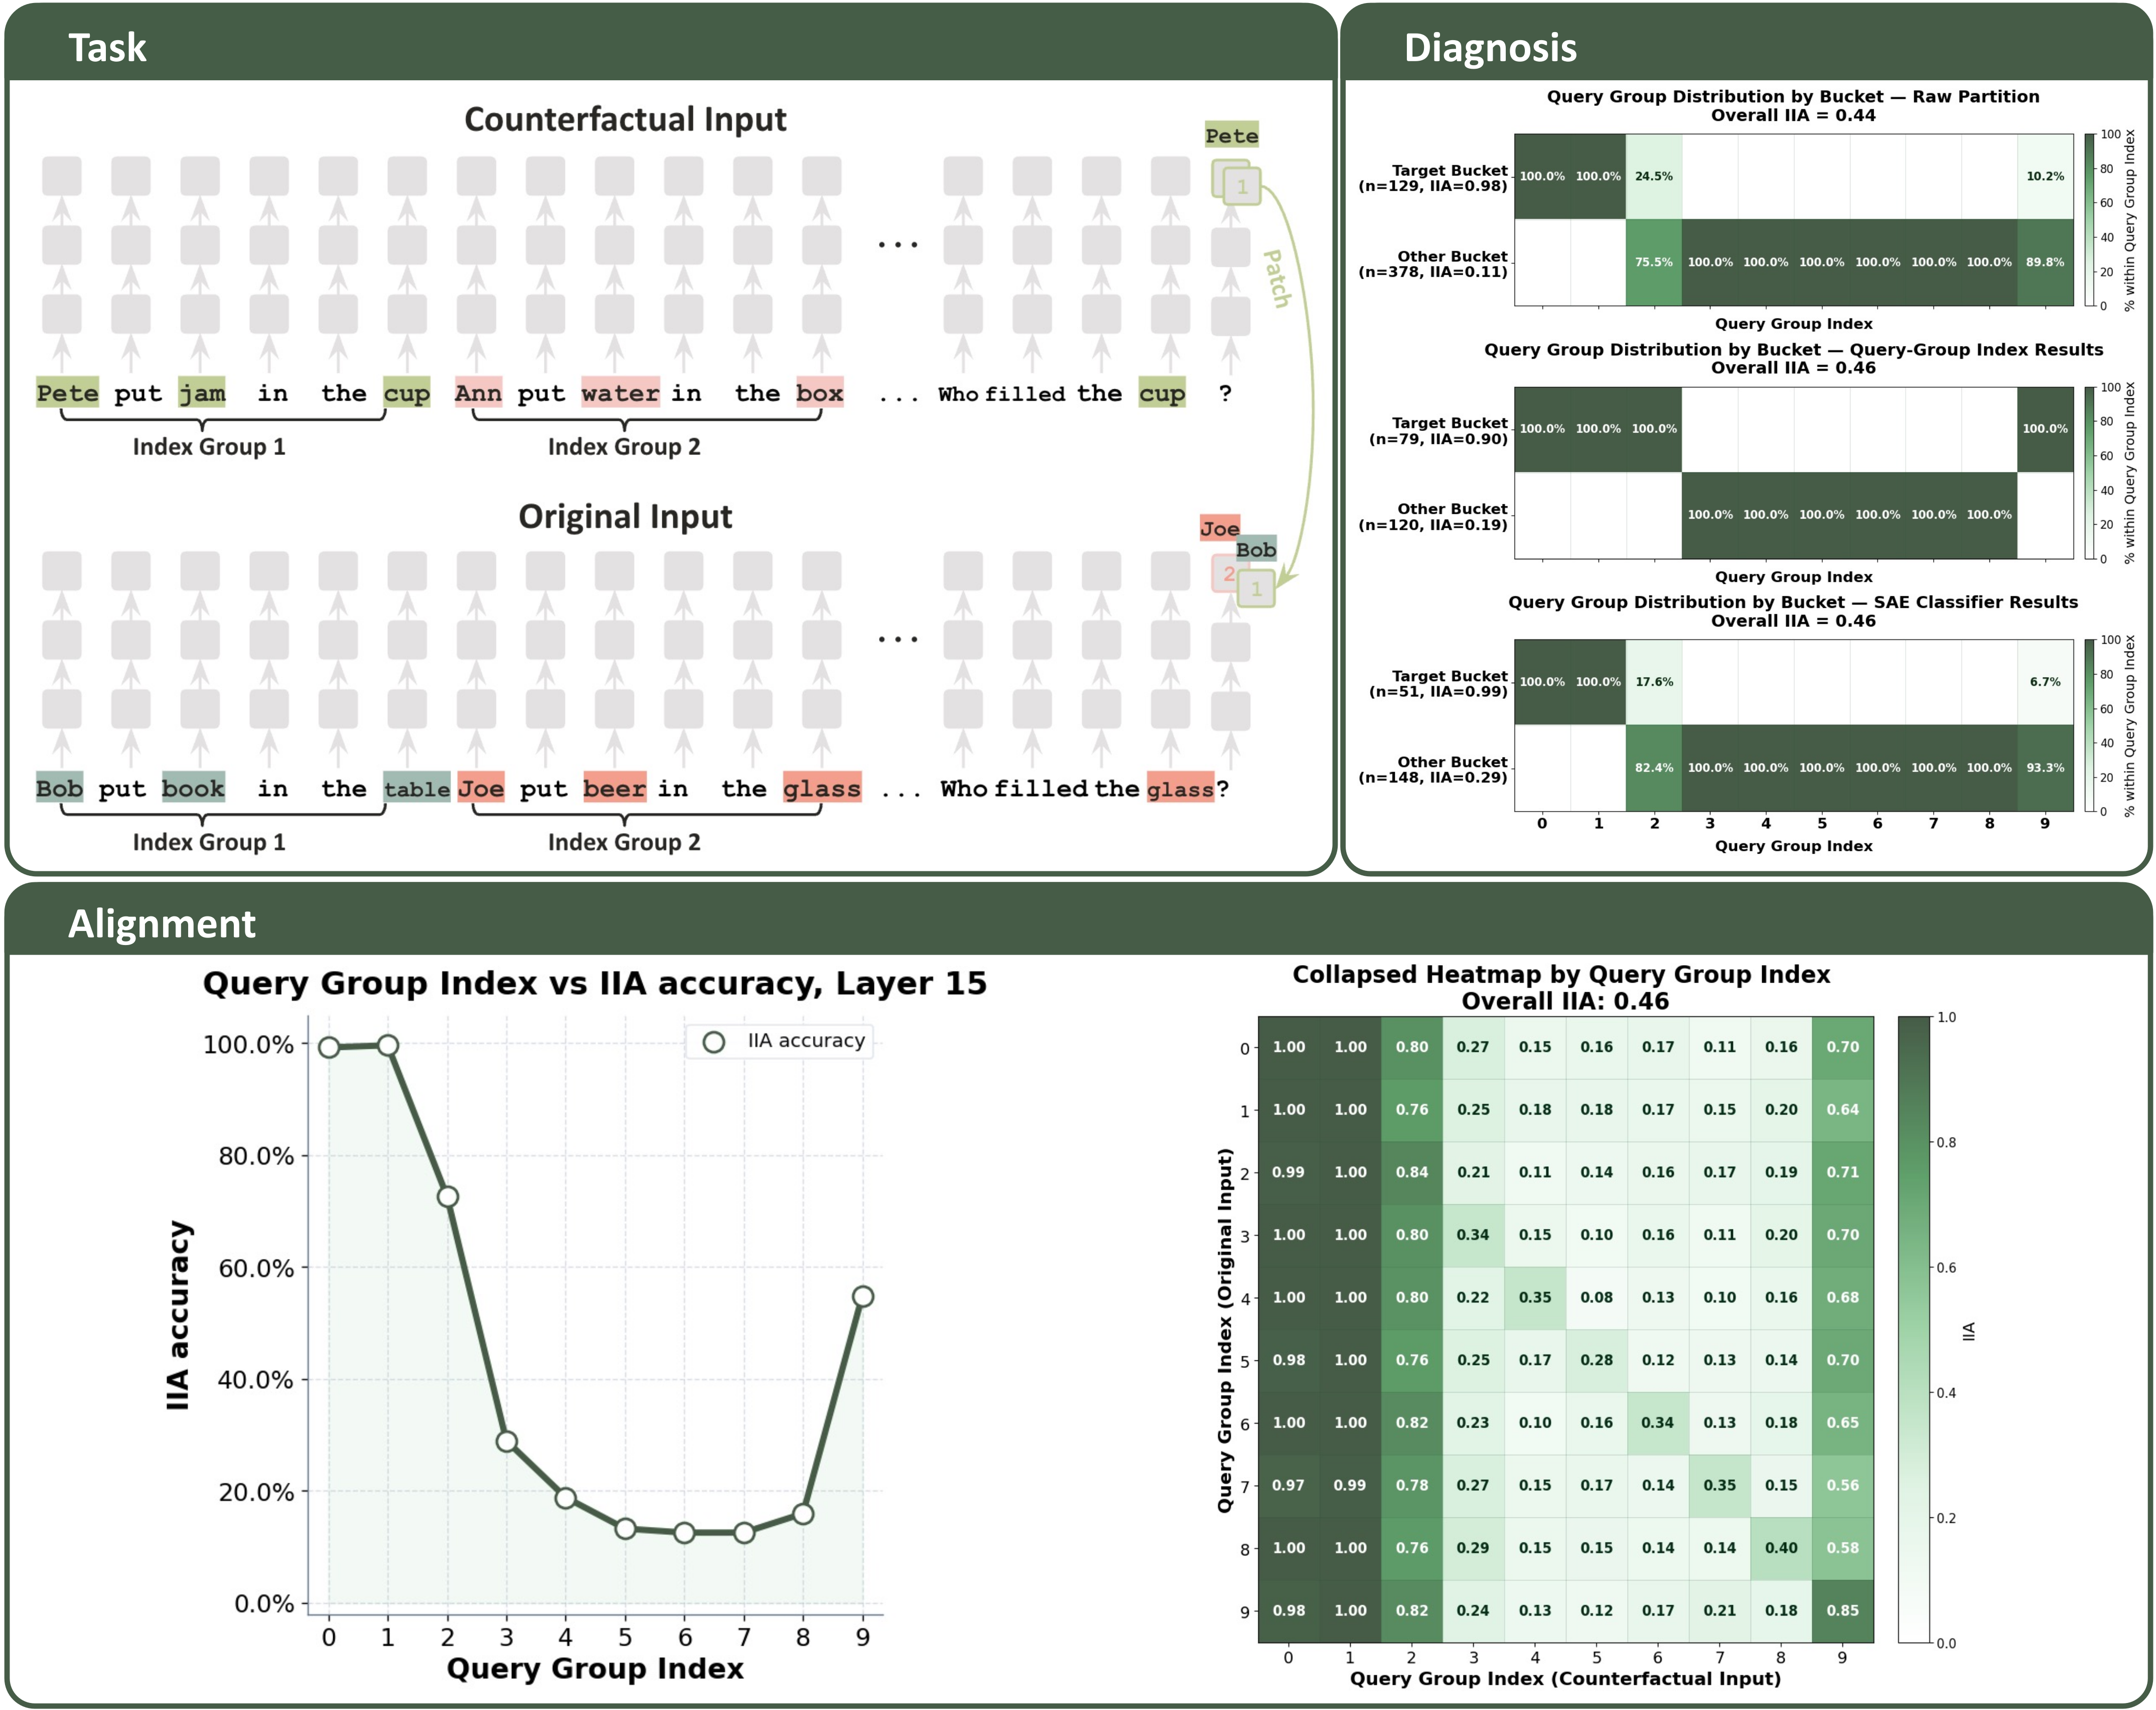
\includegraphics[width=\linewidth]{figs/entity_binding_new.png}
    \caption{\textbf{Diagnosis of the Entity Binding Task in Gemma-2-2B-Instruct.} \textbf{Top Left:} The entity-binding task evaluates in-context retrieval from sequences of templated groups (e.g., ``John fills a cup with beer...''). A query (e.g., ``Who filled a cup?'') then requests an entity from a specific group. We test a \emph{positional hypothesis}: retrieval is mediated by a high-level variable $q_{group}$ representing the queried group’s context position. The model must identify this position and dereference it to retrieve the target entity. \textbf{Bottom:} Preliminary evaluation via full-vector patching at layer 15 reveals a U-shaped alignment curve as in \citet{gur2025mixing}. \textbf{Top Right:} Our procedure constructs an interchangeability graph to isolate the well-interpreted and under-interpreted regions. This principled diagnosis recovers the failure mode automatically: the target bucket is dominated by edge groups ($q_{group} \in \{0, 1, 2, 9\}$), while the other bucket contains medial groups ($q_{group} \in \{3, 4, 5, 6, 7, 8\}$). }
    \label{fig:Entity Binding}
\end{figure}

\textbf{Task and input space.}
We evaluate our framework using the entity-binding task \citep{geiger2020neural,gur2025mixing}, where a model must retrieve specific entities from a sequence of templatic \emph{entity groups}. We test the \emph{positional hypothesis}—the idea that retrieval is mediated by a high-level variable $q_{\mathrm{group}}$ representing the context position of the queried group—using the \texttt{filling\_liquids} task with \texttt{Gemma-2-2B-Instruct}. Working within a 10-group input space $\mathcal{I}$ (where task accuracy exceeds $98\%$), we leverage this setup (Fig.~\ref{fig:Entity Binding}) to diagnose the model's internal positional mechanism. The input space $\mathcal{I}$ comprises these correctly answered prompts, annotated by the queried group position and the fixed within-group roles.

% We evaluate our framework in a more realistic in-context retrieval setting using the entity-binding task family \cite{gur2025mixing}. In this paradigm, an input consists of a sequence of \emph{entity groups}, each containing a tuple of entities that jointly instantiate a templatic clause, followed by a query requesting the retrieval of a specific entity from a targeted group. The corresponding \emph{positional hypothesis} posits that retrieval is mediated by a single high-level variable $q_{\mathrm{group}}$, which represents the context position of the queried entity group. Under this hypothesis, the model first identifies the group position and subsequently dereferences that position to retrieve the target entity.


% We instantiate this setup using the \texttt{filling\_liquids} task with a pretrained \texttt{Gemma-2-2B-Instruct} model. Each prompt contains 10 entity groups with three entities per group (e.g., \emph{``John fills a cup with beer... Who filled a cup?''}). Within this template, the queried and target entities occupy fixed within-group roles, while the queried group index varies across instances. 

\textbf{Alignment and Preliminary Evaluation.}
We replicate the positional-hypothesis experiment from \citet{gur2025mixing}, defining a high-level model where a single variable, $q_{\mathrm{group}}$, represents the queried group's position. We localize the corresponding low-level site using vanilla patching and evaluate the hypothesis via full-vector patching at the final query position. Our preliminary results at layer 15 reveal a sharply non-uniform alignment curve, shown in Fig~\ref{fig:Entity Binding} , successfully reproducing the U-shape reported by \cite{gur2025mixing}. The positional mechanism is highly faithful for entity groups at the sequence's edges but degrades significantly for those in the middle. Because the resulting global IIA is neither near-perfect nor near-chance, the aggregate scalar summary fails to characterize the specific input subspaces where the interpretation remains valid. This ambiguity underscores the need for a diagnostic procedure to isolate the well-interpreted regions of the input space.

\textbf{Bucketing the Input Space.}
We apply our partitioning procedure to the positional abstraction $(\mathcal L, \mathcal H_{\mathrm{pos}}, \Pi)$. The overall density of the interchangeability graph is $24\%$, signaling that the abstraction is far from uniformly faithful across the entire input space. Upon partitioning this graph, a clear semantic pattern emerges (Fig~\ref{fig:Entity Binding} Upper Right). The well-interpreted bucket is dominated by inputs where the queried group is located at the start or end of the sequence, while the bad bucket is dominated by inputs in the middle. This diagnosis recovers the failure mode identified manually in \citet{gur2025mixing}. The strength of our method is that this conclusion emerges directly from the structure of the intervention graph itself. Rather than manually inspecting per-index intervention curves, we obtain a principled partition of the input space into well-interpreted and under-interpreted regions. 

\textbf{Generalization through classifier.}
To test whether this partition generalizes beyond the finite graph used for bucketing, we train classifiers to predict bucket membership for unseen in-distribution inputs. We train classifiers on both the queried group index and internal SAE features. The index-based classifier recovers an interpretable rule—assigning $q_{\mathrm{group}} \in \{0,1,2,9\}$ to the target bucket and $\{3, \dots, 8\}$ to the other bucket—attaining $90\%$ IIA with $81\%$ density (Fig~\ref{fig:Entity Binding}, middle right). The SAE-based classifier further improves this to $98\%$ IIA at $97\%$ density (Fig~\ref{fig:Entity Binding}, bottom right). That internal features outperform hand-labeled features suggests the distinction between inputs in different buckets is fundamentally encoded within the model's own representations.

\textbf{Takeaway.}
This experiment demonstrates our framework's ability to transform known mechanistic failures into reusable diagnostic objects. While the initial steps replicate the positional abstraction in \cite{gur2025mixing}, our bucketing procedure reveals that the hypothesis is not merely "imperfect" on average, but highly faithful on a structured subset while systematically unfaithful elsewhere. By generalizing this boundary to unseen inputs via classifiers, we find that internal SAE features outperform hand-labeled features. This recipe moves beyond reproducing known failure modes to effectively localize, characterize, and operationalize the boundaries of model interpretations.
% This experiment shows that our method can recover a known failure mode of an existing mechanistic hypothesis 
% and turn it into a reusable diagnostic object. By design, the first two steps replicate the positional 
% abstraction experiment of \cite{gur2025mixing}; the new information comes from the last two steps. Bucketing 
% reveals that the positional hypothesis is not simply ``imperfect on average,'' but rather highly faithful 
% on a structured subset of inputs and systematically unfaithful on another. The classifier then generalizes 
% this diagnosis to unseen inputs and shows that the boundary between the two regions can be predicted both 
% from explicit semantic features and from internal SAE features, with the latter performing better. In this 
% sense, the experiment does more than reproduce the conclusion that positional retrieval fails in the middle: 
% it demonstrates that our recipe can \emph{localize} where an interpretation holds, \emph{characterize} the 
% inputs on which it breaks, and \emph{operationalize} that distinction for future inputs.

% \subsection{Entity Binding}

% We next consider a more realistic setting involving entity binding, building on prior work on in-context retrieval mechanisms. We evaluate a pretrained Gemma-2-2B-Instruct model on a task where the model is given a sequence of factual statements (e.g., ``John loves tea'', ``Mary loves cola'') followed by a query such as ``Who loves cola?''. The model achieves over $98\%$ accuracy, and we again restrict to correct predictions.

% Following prior work, we construct counterfactual inputs by swapping entity groups and evaluate causal abstraction using full vector patching. The resulting IIA is far from uniform across inputs, indicating that the hypothesized mechanism does not apply equally in all cases.

% Applying our partitioning method reveals a clear structure in the input space. Inputs where the queried entity appears near the beginning or end of the sequence form a high-density region with strong interchangeability, while inputs with middle positions fall into a low-density region. This pattern is consistent with previous findings that positional retrieval mechanisms degrade for longer-range dependencies, but here it emerges directly from the structure of interchange interventions without requiring manual inspection.

% To test whether this structure generalizes, we train classifiers to predict subset membership. A simple classifier based on the query position already separates the two regions effectively, while a classifier based on internal representations (SAE features) achieves even stronger separation. This suggests that the distinction between well- and under-interpreted inputs is both externally observable and internally encoded.

% Overall, this experiment shows that our method can recover known failure modes of a mechanism and provide a principled way to localize where a given abstraction holds.

\subsection{Entangled Factual Recall}

\begin{figure}[t]
    \centering
    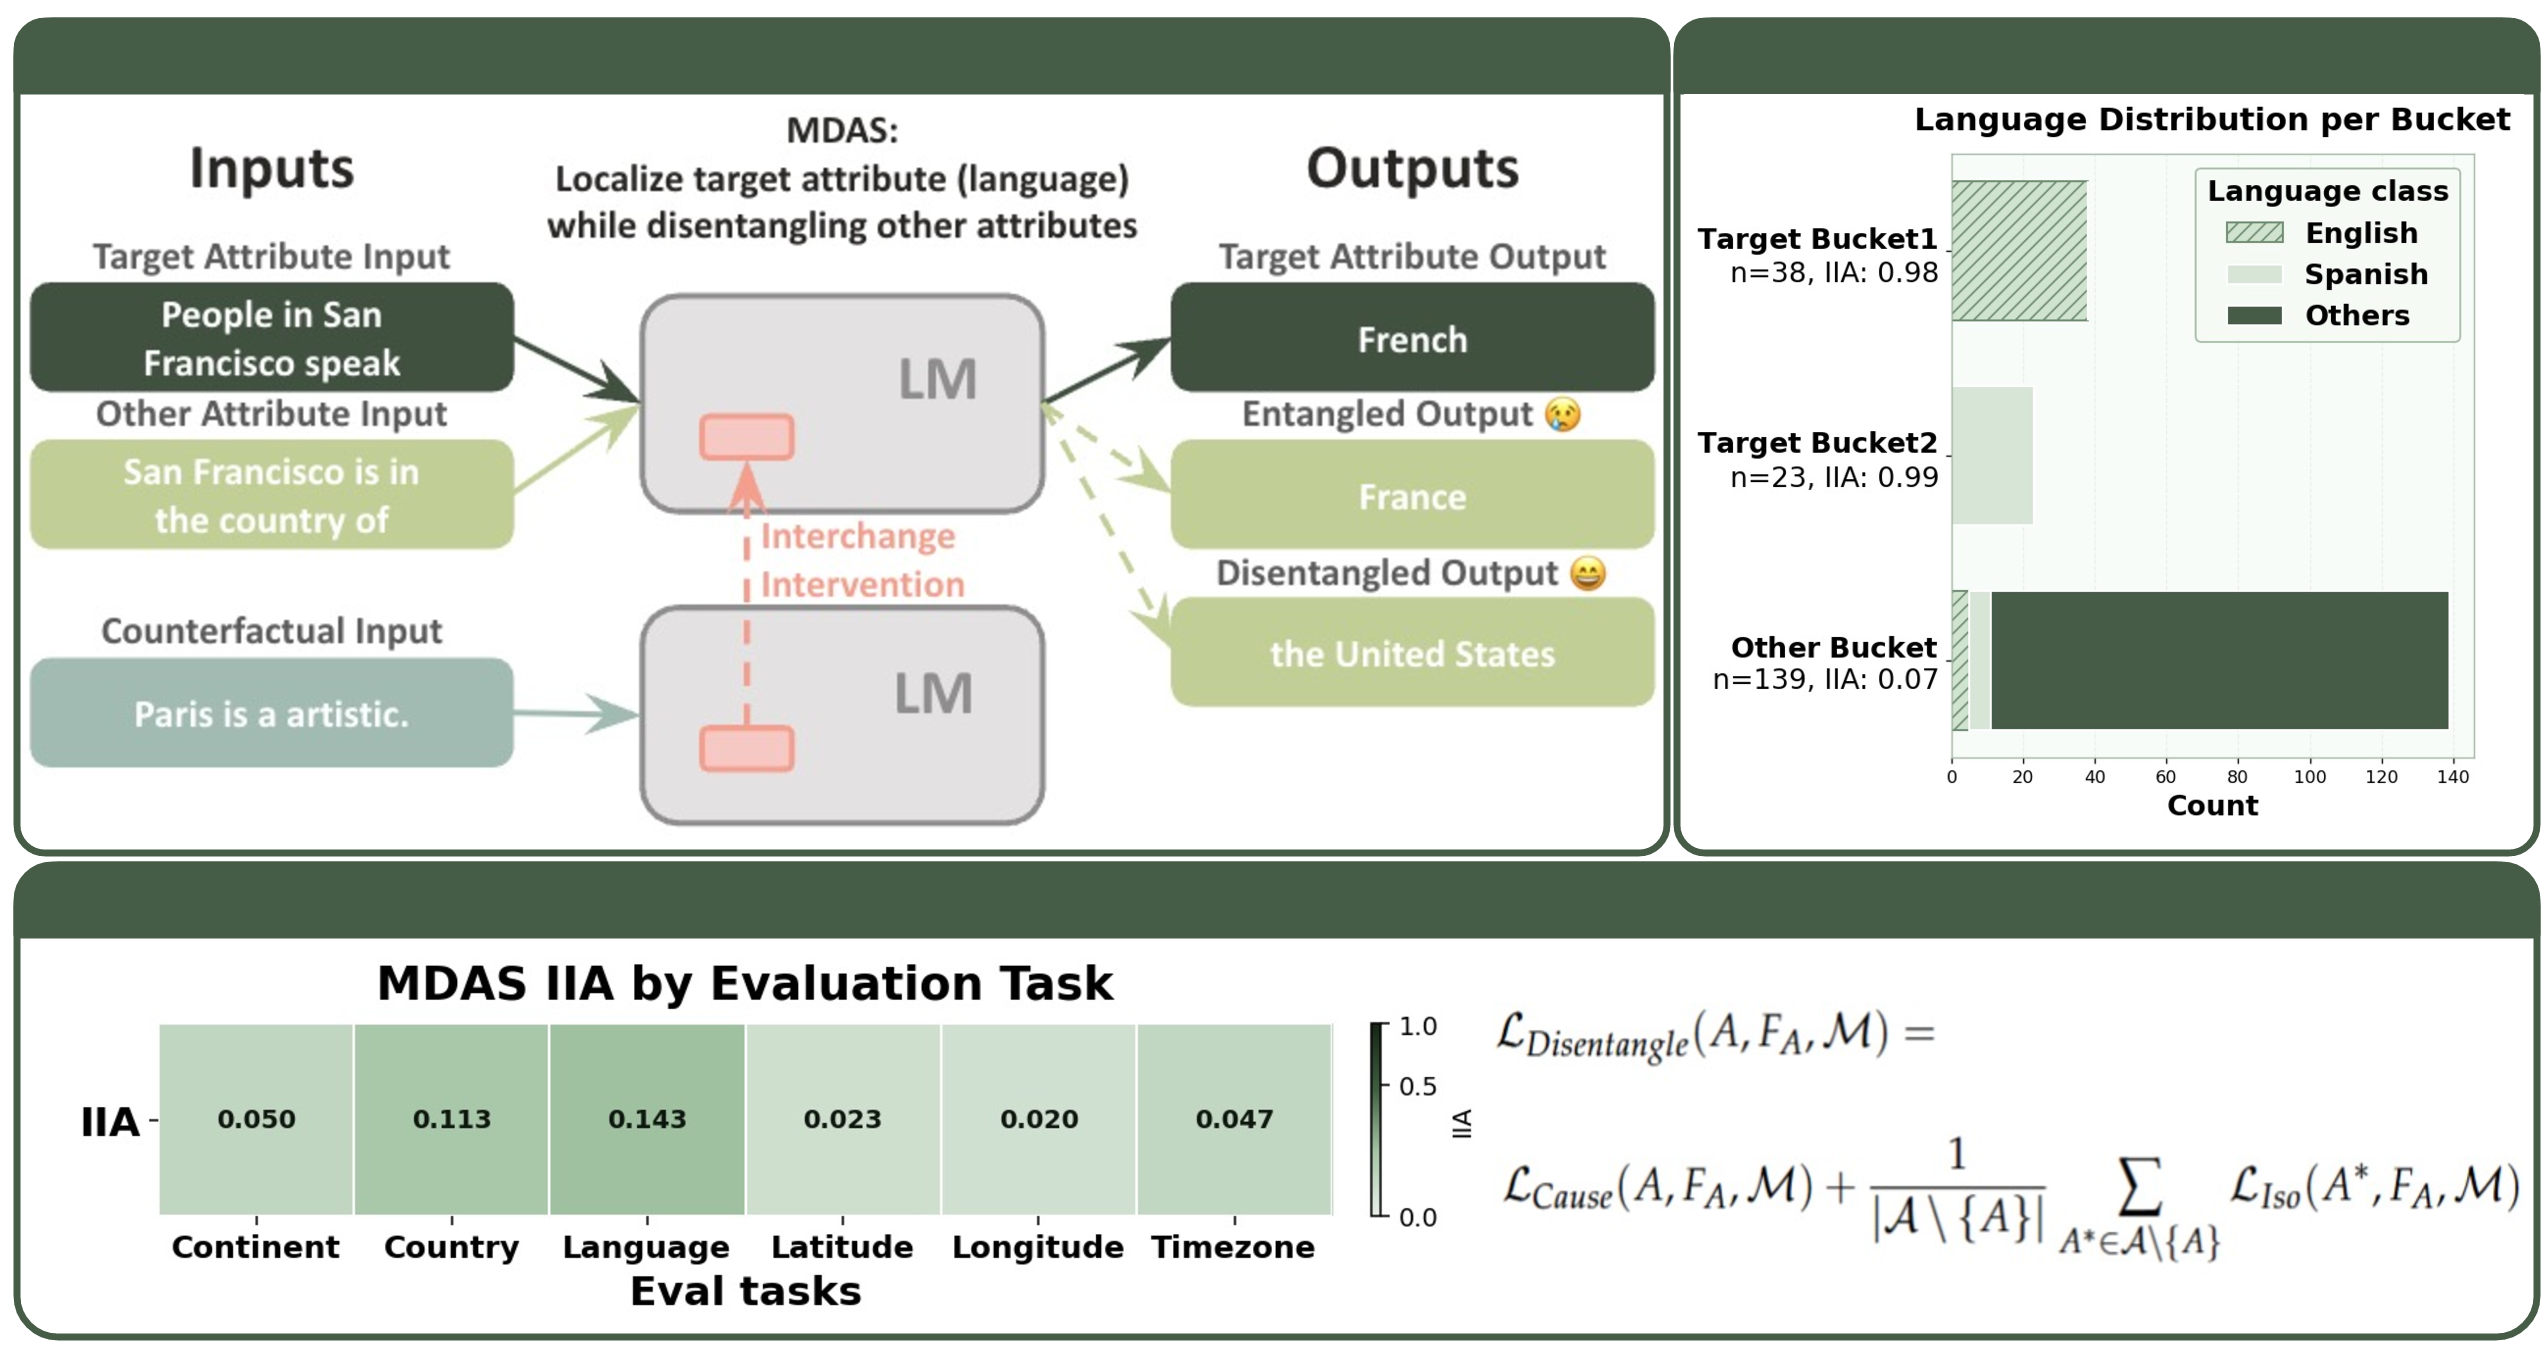
\includegraphics[width=1\linewidth]{figs/entangled_new.png}
    \caption{\textbf{Entangled Factual Recall Task and Diagnosis.} \textbf{Top Left:} This task utilizes the RAVEL benchmark to evaluate whether a specific entity attribute (e.g., \textsc{Language}) can be isolated from other co-encoded attributes like \textsc{Country}, \textsc{Continent}, and \textsc{Timezone}. It is particularly challenging because these features are often entangled within a single internal model state, making surgical intervention difficult. \textbf{Bottom:} MDAS Results. We train the alignment using all samples from all attributes to isolate the \textsc{Language} attribute and evaluate it on all attributes.  \textbf{Top Right:} After partition, the "Target Buckets" correspond to regions where the representation is highly faithful for specific languages—English and Spanish—while the "Other Bucket" captures the remaining modes.}
    \label{fig:factual}
\end{figure}

\textbf{Task and input space.}
We evaluate our framework on \emph{entangled factual recall} using the RAVEL benchmark \citep{huang2024ravel}. This task tests the ability of interpretability methods to isolate a specific entity attribute from others co-encoded in the same representation (\cref{fig:factual}). This task is particularly challenging because attributes are often entangled within a single internal state, making it difficult to intervene on one without affecting others. Using a pretrained \texttt{Llama-3.1-8B} model, we focus on isolating the \textsc{Language} attribute from others. 

\textbf{Alignment and Preliminary Evaluation}
A successful alignment in the \textsc{Ravel} benchmark must satisfy two key properties: {causal effectiveness} and {isolation}.For a target attribute $X \in \mathcal{A}$ and its aligned representation $\Pi_X$ mapped via $\tau_X$, a high \textbf{Cause} score signifies that an interchange intervention $II(\mathcal{M}, s, \Pi_X)(b)$ successfully propagates the attribute value $\tau_X(s)$ from the source $s$ into the model's output for the base input $b$. Conversely, a high \textbf{Iso} (isolation) score ensures the intervention is surgically precise, remaining invariant to the states of extraneous features $Y \in \mathcal{A} \setminus \{X\}$. The formal loss objectives are detailed in (\ref{eq:loss_cause}) and (\ref{eq:loss_iso}) in the appendix. While Multi-task Distributed Alignment Search (MDAS) is architected to jointly optimize these criteria, the resulting alignment yields a held-out Interchange Intervention Accuracy (IIA) of only 14.3\%. This discrepancy identifies a central theoretical puzzle: despite MDAS being explicitly designed for attribute disentanglement , the learned subspace remains a fragile abstraction. This failure points to a structural mismatch that aggregate metrics cannot illuminate, necessitating our partitioning method to diagnose why the alignment fails to generalize beyond the training distribution

\textbf{Bucketing the input space.}
We next apply our bucketing procedure to the learned MDAS language subspace. The resulting intervention  graph is sparse overall, with edge density only about \(10\%\). Once we partition this graph, however, a clear structure emerges (Fig~\ref{fig:factual} right). The dense buckets correspond almost exactly to single-language regions: one 
bucket is dominated by English-speaking cities and Spanish-speaking cities, each with high IIA (around \(98 \%\)). The remaining cities fall into a diffuse ``other languages'' bucket with very low IIA. This shows that the learned MDAS subspace does not faithfully represent the \textsc{Language} attribute in general. Instead, it collapses the input space into a small 
number of coarse language-specific clusters, preserving interchangeability mainly within the same language while failing on cross-language interventions. 

\textbf{Generalization through classifier.}
To test generalization, we train an SAE-based classifier to predict bucket membership for unseen inputs. The classifier reproduces the partition with $90\%$ accuracy, confirming that the language-specific structure is indeed encoded in the model's internal representations. Inspecting the highest-weight SAE features reveals only weak signals that are loosely consistent with the corresponding languages. These signals are far less direct than the buckets themselves: while reading SAE feature descriptions provides only weak, post hoc evidence, examining the grouped inputs in each bucket makes the underlying structure immediately clear.

% We further inspect the highest-weight SAE features used by the classifier in order to understand what distinguishes the buckets. This analysis does recover weak language-specific signals: for example, once a bucket is already known to correspond to English- or Spanish-speaking cities, one can identify SAE features whose interpretations are loosely consistent with that language. However, these signals are much less direct than the buckets themselves. In practice, reading off feature descriptions from SAE dashboards provides only weak and highly post hoc evidence about what a bucket represents, whereas directly examining the inputs grouped into each bucket makes the structure immediately clear.


% \textcolor{red}{(To be refined.)}

\textbf{Takeaway.}
This experiment reveals a limitation of MDAS-style disentanglement in the entangled factual recall setting. Although MDAS is designed to isolate the target concept from correlated non-target attributes, our analysis shows that it can do so only by \emph{collapsing the target representation} itself. The resulting subspace is partially isolated but only weakly faithful: it preserves coarse within-language structure while losing the finer-grained information needed for robust cross-language interchangeability. In this case, bucketing makes the failure mode explicit by showing that the learned representation separates a few major language clusters rather than capturing the \textsc{Language} attribute as a whole.

% Finally, we study a challenging setting involving entangled representations, based on the RAVEL benchmark. We evaluate a pretrained LLaMA-3.1-8B model on factual recall tasks involving multiple attributes of entities (e.g., language, country, latitude). We focus on the language attribute and restrict to inputs where the model predicts correctly.

% We apply multi-dimensional alignment search (MDAS) to learn a shared representation across attributes. While MDAS achieves reasonable alignment for some attributes, the language variable exhibits very low IIA (around $17\%$), suggesting a significant mismatch between the high-level variable and the learned representation.

% Applying our partitioning method reveals a striking and highly structured pattern. When we divide the input space into a small number of clusters, each high-density cluster corresponds almost entirely to a single language (e.g., English, Spanish, Russian), while cross-language pairs fall into low-density regions. Increasing the number of clusters refines this structure, progressively isolating individual language groups.

% This indicates that the learned representation is only locally consistent: it supports correct interventions within a language group but fails to generalize across groups. In other words, the low IIA is not due to random noise, but to systematic information loss caused by entanglement across attributes.

% We further train a classifier based on SAE features to predict cluster membership. While the classifier successfully separates the clusters, analysis of the features shows that signals distinguishing different languages are relatively weak compared to shared language-related features. This suggests that the representation encodes language information, but in a compressed or entangled form that does not fully support counterfactual reasoning.

% Taken together, these results demonstrate that our method can uncover structured failure modes that are invisible to aggregate metrics, and can diagnose when an alignment method fails due to representational limitations rather than hypothesis mismatch.

% \subsection{Summary}

% Across all three settings, partitioning the input space provides a consistent and informative view of causal abstraction. Rather than treating IIA as a single scalar metric, our method reveals where an abstraction is exact, where it fails, and why. This enables a more fine-grained evaluation of hypotheses and, importantly, provides concrete guidance for improving them.
